\chapter{Návrh desek plošných spojů}

Návrh PCB (desek plošných spojů) byl proveden podle výrobních pravidel firmy JLCPCB\footnote{\url{https://jlcpcb.com}}. Maximální rozměry pro levnou výrobu (2 až 4\$ za 5~ks desek) jsou $\SI{100}{}\times \SI{100}{\milli\metre}$ pro dvouvrstvou desku. Do těchto výrobních možností je tedy nutné koncipovat veškeré návrhy desek. Desky budou navrženy pro ruční osazení a jsou tomu tedy i uzpůsobeny pouzdra součástek. Tuto cestu jsem zvolil, protože i po započítání nákladů na dopravu a clo je výroba u této společnosti nesrovnatelně cenově výhodnější, než u české konkurence. Veškeré návrhy PCB a schémat jsou provedeny v programu KiCad\footnote{\url{https://kicad.org/}}, který je dostupný zdarma a~lze jej používat i~pro komerční projekty. Navíc je open-source a má veřejně dostupné Python API (Application Programming Interface), což umožňuje komunitě vytvářet pluginy a rozšíření pro usnadnění práce.

\section{Návrh desky plošných spojů nabíječky}

Po návrhu schematického zapojení samotného nabíjecího obvodu bylo zapotřebí navrhnout desku plošných spojů. Jelikož se jedná o jednoduchý obvod s málo součástkami, vystačí dvouvrstvá deska plošných spojů. Na desce jsou navrženy celkem tři druhy možností napájení. Je zde konektor Micro-USB, USB-C a také dvě plošky pro připojení jakéhokoli zdroje \SI{5}{} až \SI{40}{\volt}. Poslední ze zmíněných možností se hodí právě pro připojení jakéhokoliv solárního panelu, který splňuje bude mít dostatečný výkon. Společně s možností solárního panelu je zde také umístěna pájecí propojka, kterou lze zapnout nebo vypnout MPPT funkci obvodu. Pokud uživatel chce funkci vypnout (napájení ze stabilního zdroje napětí), stačí pájením spojit prostřední plošku a plošku s nápisem OFF. Při zapnutí je třeba doplnit dva rezistory do napěťového děliče (R10 a R11 podle schématu \ref{fig_ChargerSchematic}) dle rovnice \ref{eq_MPPTRegulator}. Pro připojení nabíječky k hlavní desce jsou použity \SI{2}{\milli\metre} banánky, které zajistí mechanické zajištění a navíc snesou proudové zatížení až \SI{15}{\ampere}, takže nebudou vznikat ztráty přechodovým odporem. Při návrhu spojů bylo dbáno na optimální rozložení součástek z hlediska proudových smyček dle datasheetu výrobce čipu. Výsledná deska má rozměry $\SI{40}{}\times \SI{40}{\milli\metre}$ a je vidět na obrázku \ref{fig_chargerBoardKiCad}.

\begin{figure}[h]
    \centering
    \subfloat[][3D model desky plošného spoje]{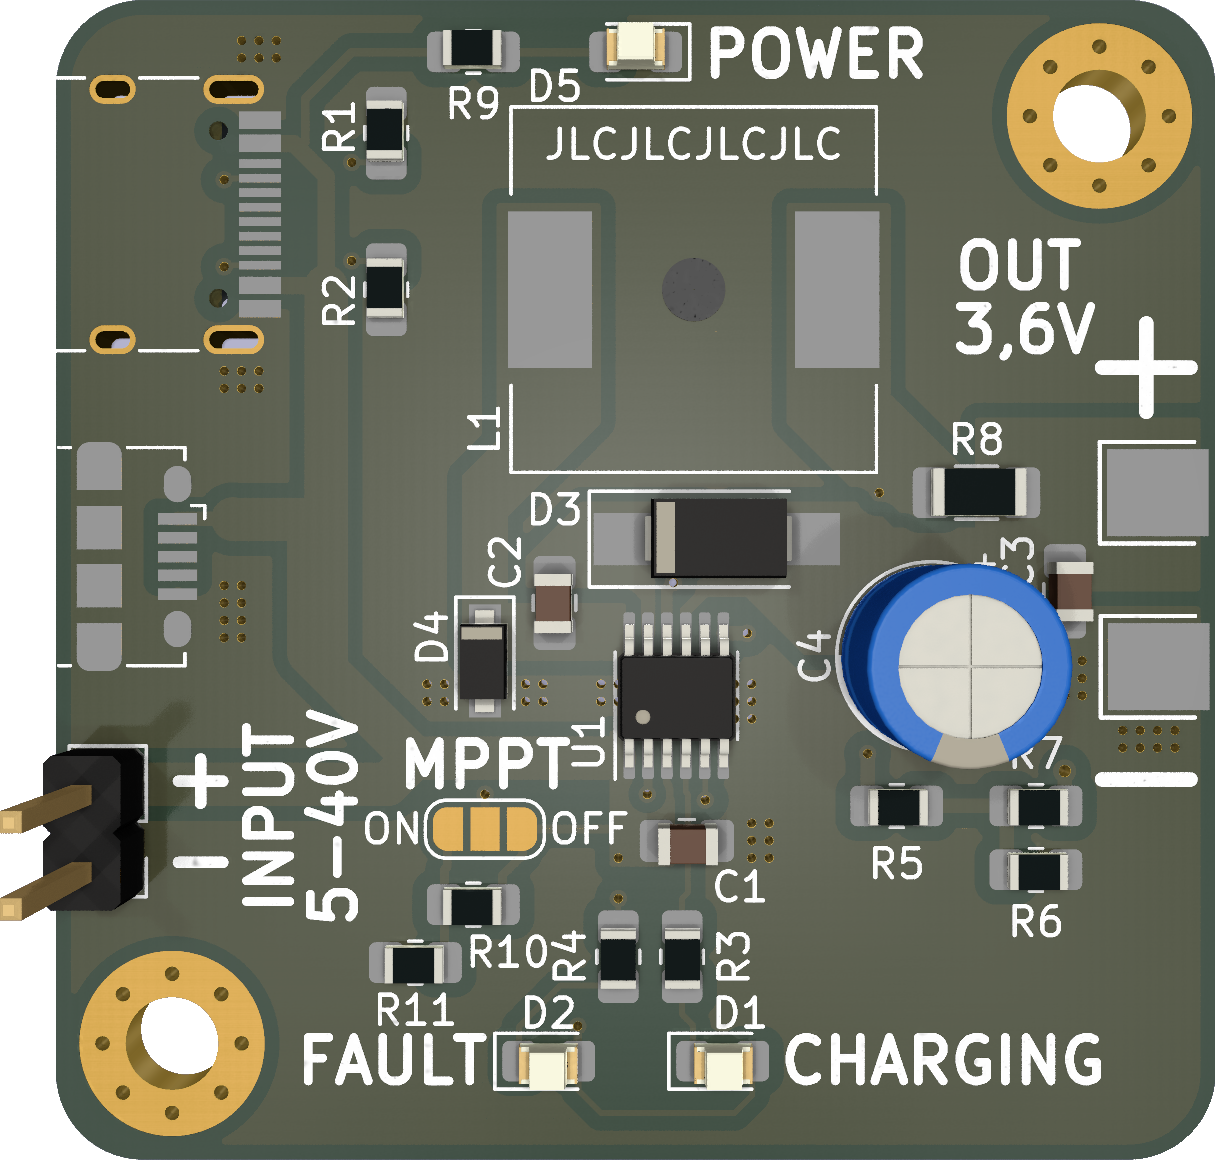
\includegraphics[width=0.41\textwidth]{obrazky/batteryCharger-top_.png}}
    \subfloat[][Vyrobená a osazená deska plošného spoje]{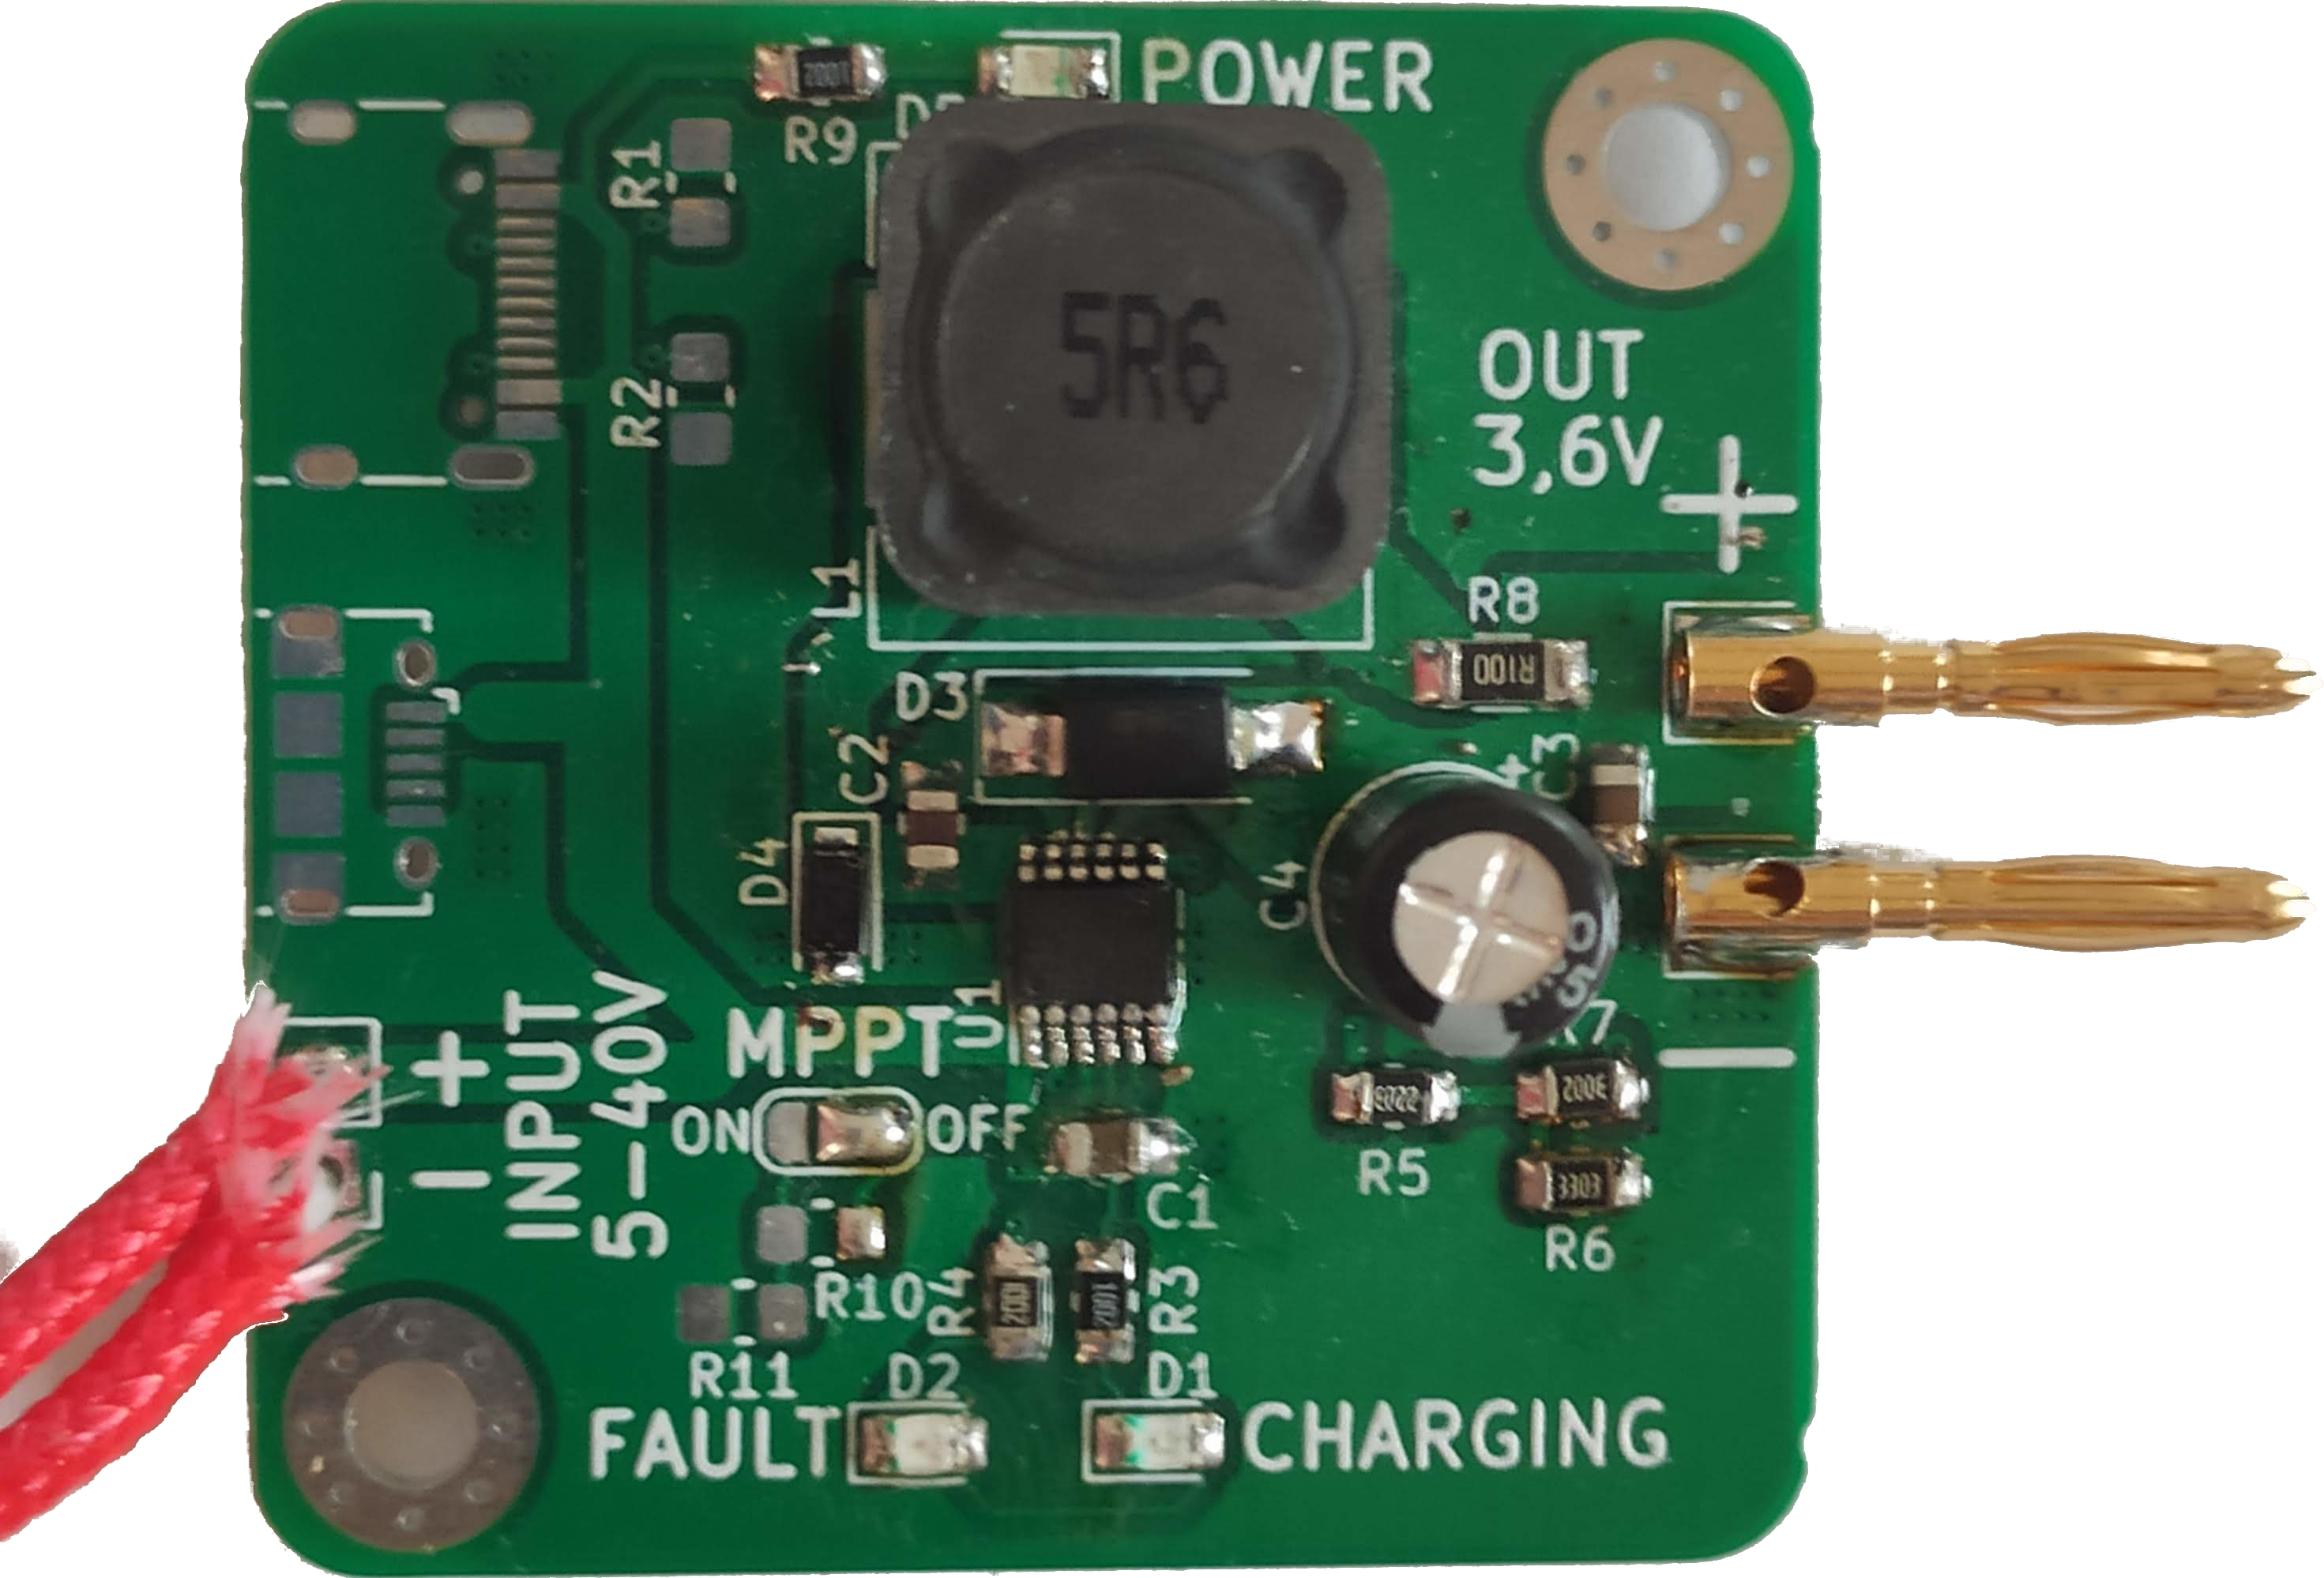
\includegraphics[width=0.59\textwidth]{obrazky/batteryCharger-final.png}}
    \caption{Deska plošných spojů pro nabíječku.}
    \label{fig_chargerBoardKiCad}
\end{figure}

\section{Návrh desky plošných spojů hlavní desky}

Po návrhu celkového blokového schématu \ref{fig_BlockDiagram-full} je potřeba provést návrh desky i pro hlavní řídící desku. Tato deska bude rozdělena do dvou, jedna s veškerou elektronikou a většinou senzorů a druhá menší se senzorem intenzity osvětlení a senzorem UV záření. Toto rozdělení je provedeno kvůli možnosti umístění senzorů světla z hlediska mechanické konstrukce na místo, kde nebudou stíněny. Obě dvě tyto desky jsou koncipovány jako dvouvrstvé. Na hlavní desce je převážná většina součástek umístěna na přední straně a na zadní jsou umístěny víceméně ostatní senzory. Deska obsahuje také čtyři LED pro indikaci funkce jednotlivých napájecích větví, tyto LED jsou nezávisle na sobě zapínatelné pomocí pájecí propojky. Programování probíhá pomocí externího programátoru CP2102\footnote{\url{https://www.silabs.com/interface/usb-bridges/classic/device.cp2102}}, který se připojuje k hlavní desce na které jsou pouze dva tranzistory a rezistory potřebné k zajištění přepínání ESP32 do režimu nahrávání firmware. Dále deska obsahuje již zmíněný LoRa modul RFM95W ke kterému lze připojit připájením \SI{100}{\nano\farad} kondenzátoru anténu osazenou přímo na desce nebo U.FL konektor pro připojení externí antény. Celá deska je navržena s ohledem na co nejnižší spotřebu a pro dosažení co nejlepších parametrů bylo dbáno na doporučené zapojení dle datasheetu výrobců. Největší pozornost byla věnována oblasti spínaného zdroje, jelikož je zde potřeba správně rozložit součástky a dimenzovat spoje na desce a také oblasti okolo mikropáskového vedení do k anténám, kde je potřeba minimalizovat rušení a také přizpůsobit spoje na impedanci \SI{50}{\ohm}.

Na menší desce se světelnými senzory jsou umístěny pouze součástky podle datasheetů od výrobců a také konektory pro připojení k hlavní desce. Budou využity tzv. pin headery na kterých je vyvedeno napájení \SI{3.3}{\volt}, analogový výstup ze senzoru UV záření a také signály datové sběrnice I$^2$C.



% Deska plošných spojů byla navržena podle výrobních pravidel firmy JLCPCB\footnote{https://jlcpcb.com/}. Maximální rozměry jsou $\SI{100}{}\times \SI{100}{\milli\metre}$ a~byla využita dvouvrstvá deska. Do těchto výrobních možností je tedy nutné koncipovat celý návrh desky plošných spojů. Osazování proběhne v~drtivé většině součástek u~dříve zmíněné firmy strojně, jelikož i~za cenu včetně osazení je cena součástek nakoupená právě u~nich nesrovnatelná například s~českou konkurencí. Jednou z~možných nevýhod je absence strojního osazení z~obou stran desky, tento výrobce umožňuje osazovat pouze jednu stranu desky plošného spoje.

% Pro dosažení co nejlepších parametrů celého obvodu bylo dbáno na doporučené zapojení dle datasheetu výrobců. Největší pozornost byla věnována oblasti spínaného zdroje, jelikož zde je důležité správně rozložit součástky a~dimenzovat spoje na desce. Pro dosažení nízké spotřeby je možné jednotlivé skupiny senzorů a~modulů vypínat. Na obrázku \ref{fig_PCB-top} je vidět celá navržená deska plošných spojů o~rozměrech $\SI{100}{}\times \SI{100}{\milli\metre}$ z~horní strany. Výsledná deska plošných spojů byla navržena v~programu KiCad\footnote{https://www.kicad.org/}, který je dostupný zdarma a~lze jej používat i~pro komerční projekty.

% \begin{figure}[h]
%     \centering
%     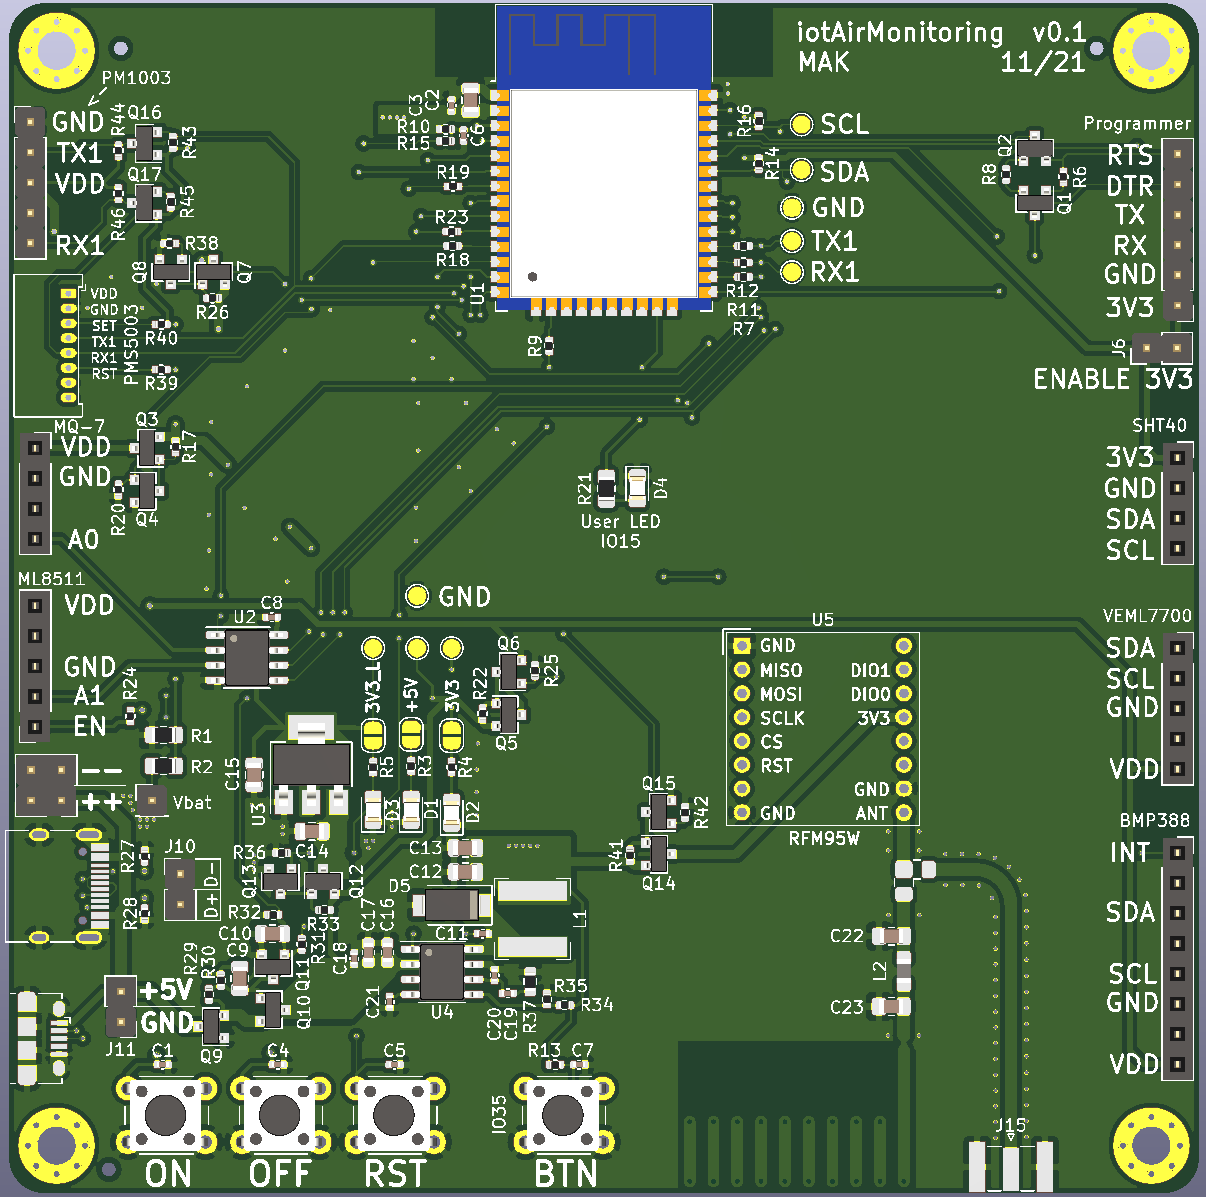
\includegraphics[width=0.7\textwidth]{obrazky/PCB_top.png}
%     \caption{Pohled na 3D model desky plošného spoje shora.}
%     \label{fig_PCB-top}
% \end{figure}